\documentclass[10pt]{article}
\usepackage[T1]{fontenc}
\usepackage{lmodern, amsmath, amssymb, graphicx, hyperref}
\usepackage[margin=.74in]{geometry}
\setlength{\parindent}{0pt}\setlength{\parskip}{7pt}
\begin{document}
\begin{center}{\Large Constructed fixed-width Boolean arithmetic}\\[4pt]
Local successor --- 15 November 2026\end{center}
\textbf{Result and evidence.} Three accepted local stages: draft045/244 statements, 
draft047/252 and draft048/262, each including prior work, exit0/no warnings.
Data PCC-20261115-bc3f62, f67070, b6b5e0 with receipts023, 024, 025 pin sources, 
compiler logs and exits, including failed044 and046. Central dependency prints
are standard; the full-adder truth identity prints no axioms. These are local
proofs outside shared Transport53/57/fresh. All records are unsigned and
not independently covered [pcc:unverified].

\textbf{Actual Boolean calls.} The full adder invokes two XOR, two AND and one
OR primitive. With Boolean inputs $a, b, c$, it computes
\[
 p=a\mathbin{\mathrm{xor}}b, \quad s=p\mathbin{\mathrm{xor}}c, \quad
 k=(a\land b)\lor(p\land c).
\]
All eight cases are proved by Lean case analysis. With $\nu$ the Boolean-to-natural
map, the identity is $\nu(a)+\nu(b)+\nu(c)=\nu(s)+2\nu(k)$.
Each actual primitive emits its event; the desired count is not merely attached
to an uninstrumented operation [pcc:unverified].

\textbf{Word recursion.} Define LSB-first decode by
\[
 D([])=0, \qquad D(b::t)=\nu(b)+2D(t).
\]
The ripple routine takes equal-length input lists $x, y$, an initial carry $c$, 
and returns output list $s$ and overflow carry $k$. The source proves
\[
 |s|=|x|=q, \qquad D(s)+2^q\nu(k)=D(x)+D(y)+\nu(c).
\]
It also proves $D(s)<2^q$, hence
\[
 D(s)=(D(x)+D(y)+\nu(c))\bmod2^q.
\]
The equal-length premise is explicit; mismatched input branches are not admitted
by these theorems. Width zero retains the incoming carry and has no Boolean
gate calls. Arithmetic identity and count statements retain overflow rather
than assuming a favorable no-carry case [pcc:unverified].

\textbf{Exact gate counts.} The actual flattened ripple trace has
$2q$ XOR events, $2q$ AND events, $q$ OR events and total length $5q$.
Those are Boolean circuit operation counts. They do not include preparation, 
list traversal, allocation, indexing, stack, constants or trace-concatenation work.
No total bit-runtime conclusion follows merely from these counts
[pcc:unverified].

\textbf{Primary sources and failed attempts.} Pinned Lean
Init/Data/BitVec/Bitblast defines standard adcb, adc, adc\_spec and add\_eq\_adc.
Pinned Nat Bits, BinaryRec, Size and division facts, and Mathlib ZMod canonical
cast identities inform the representation bridge. Standard arithmetic is
reused without a novelty claim. Failed044 had an exported-definition unfolding
issue and a missing distributive rewrite; failed046 needed consistent quotient
denominator normalization. Original sources and raw failures remain exact
[pcc:unverified].

\newpage
\begin{center}{\Large Constructed representation and signed values}\end{center}
\textbf{Construct the input.} The routine does not assume a favorable word
representation. For requested width $q$, recursively encode a natural $n$:
\[
 E(0, n)=[], \qquad E(q+1, n)=\mathrm{bodd}(n)::E(q, \lfloor n/2\rfloor).
\]
The source proves its length is $q$ and the exact decomposition
\[
 D(E(q, n))+2^q\left\lfloor\frac{n}{2^q}\right\rfloor=n, 
 \qquad D(E(q, n))=n\bmod2^q.
\]
A Word stores the actual list with a length proof. Its value is its decoded
natural cast into $\mathbb Z/2^q\mathbb Z$. The constructor has canonical value
$n$ in that ring. addWord invokes the actual ripple circuit and has value
$V(x)+V(y)$ with $5q$ emitted gates, including $q=0$ [pcc:unverified].

\textbf{Explicit negative words.} Complement invokes XOR with true at each
bit, with exactly $q$ emitted gates. It proves
\[
 D(\mathrm{invert}(x))+D(x)+1=2^q, \qquad
 V(\mathrm{invertWord}(x))=-V(x)-1.
\]
Then negateWord adds the constructed one word using the actual adder:
\[
 V(\mathrm{negateWord}(x))=-V(x), \qquad
 \#\mathrm{gates}=q+5q=6q.
\]
The signed constructor encodes a magnitude and conditionally applies this
circuit. Its value equals the canonical integer cast for zero, positive and
negative integers, and its circuit-event count is at most $6q$. This includes
the zero-width ring [pcc:unverified].

\begin{center}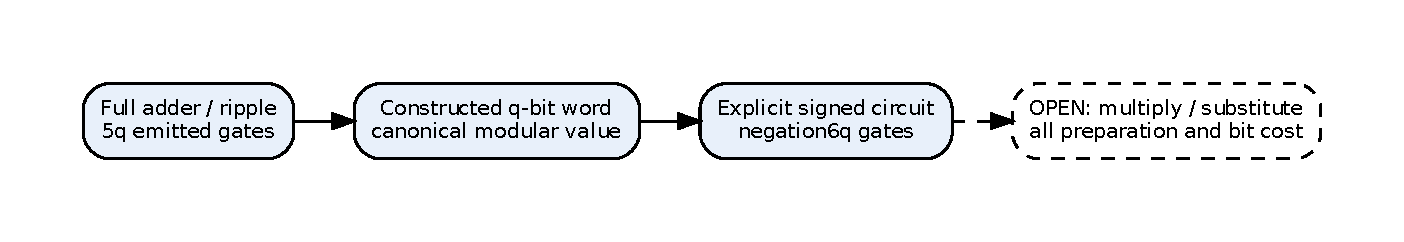
\includegraphics[width=\linewidth]{word-dependencies-001.pdf}\end{center}

\textbf{Preparation remains charged.} A positive integer constructor has zero
Boolean circuit events but still builds $q$ bits. The bodd/halving operations, 
integer representation, constants, control, list traversal, arrays, indices, 
trace/logging and retained storage have not been priced. A semantic value
bridge is not an extracted-program or instrumentation-erasure theorem.
No free representation or total cast/bit-runtime claim is made
[pcc:unverified].

\textbf{Next discriminating action.} Construct a width-preserving shift and
shift/add multiplication, retain overflow modulo $2^q$, derive actual gate counts
without sparsity assumptions, then substitute these words in actual boxed
expression evaluation. Price all scalar, input, AST, denominator, inversion, memory
and control costs. Original creation, modes, children, recursion, public relation, 
finder, extraction, retry and expected cost remain open [pcc:unverified].
\end{document}
